%%%%%%%%%%%%%%%%%%%%%%%%%%%%% Define Article %%%%%%%%%%%%%%%%%%%%%%%%%%%%%%%%%%
\documentclass{article}


%%%%%%%%%%%%%%%%%%%%%%%%%%%%% Using Packages %%%%%%%%%%%%%%%%%%%%%%%%%%%%%%%%%%
\usepackage{geometry}
\usepackage{pgfplots}
\usepackage{lipsum}
\usepackage{mdframed}
\usepackage{amsthm}
\usepackage{bm}
\usepackage{titlesec}
\usepackage{tocloft}
\usepackage{ragged2e}
\usepackage{fancyhdr}
\usepackage{glossaries}
% \usepackage[spanish]{babel}
\usepackage[sorting=none]{biblatex}

\usepackage[hidelinks]{hyperref}
\usepackage[all]{hypcap}
\usepackage{csquotes}
\usepackage{pdfpages}
\usepackage{booktabs,multirow}
\usepackage{listings}
\usepackage{dirtree}
\usepackage{eurosym}
\usepackage{indentfirst}


%%%%%%%%%%%%%%%%%%%%%%%%%% Page Setting %%%%%%%%%%%%%%%%%%%%%%%%%%%%%%%%%%%%%%%
\geometry{a4paper}
\graphicspath{{img/}}
\addbibresource{bibliography.bib}
\numberwithin{figure}{section}
\numberwithin{table}{section}
\setlength{\belowcaptionskip}{5pt} 

\titleformat{\paragraph}
{\normalfont\normalsize\bfseries}{\theparagraph}{1em}{}
\titlespacing*{\paragraph}
{0pt}{3.25ex plus 1ex minus .2ex}{1.5ex plus .2ex}

\fancyhf{}
\pagestyle{fancy}
\fancypagestyle{plain}{}
\lfoot{\thepage}
\fancyhead{}
\renewcommand{\headrulewidth}{0pt}

\lhead{PROYECTO FIN DE GRADO}

\titleformat{\section}
{\rmfamily\Large\raggedleft\uppercase}{\thesection.}{0.1cm}{}[{\titlerule[0.5pt]}]
\titleformat{\subsection}
    {\rmfamily\large\uppercase}{\thesubsection.}{0.1cm}{}

%%%%%%%%%%%%%%%%%%%%%%%%%%%%%%% Plotting Settings %%%%%%%%%%%%%%%%%%%%%%%%%%%%%
\usepgfplotslibrary{colorbrewer}
\pgfplotsset{width=8cm,compat=1.9}


%%%%%%%%%%%%%%%%%%%%%%%%%%%%%%% Title & Author %%%%%%%%%%%%%%%%%%%%%%%%%%%%%%%%
\title{Diseño de un STACK Tecnológico para un equipo de IA basado en MLOPs }
\author{Asier Villar}


%%%%%%%%%%%%%%%%%%%%%%%%%%%%%%% Components %%%%%%%%%%%%%%%%%%%%%%%%%%%%%%%%%%%
\newcommand{\listequationsname}{\Large{Índice de ecuaciones}}
\newcommand{\myequations}[1]{
    \addcontentsline{equ}{myequations}{\protect\numberline{\theequation}#1}
}
\newcommand{\blankpage}{% comando pagina vuota
    \clearpage
    \null
    \thispagestyle{empty}%
    \clearpage
}

\newcommand{\equationNote}[2]{
    \begin{align} \label{#2} \ensuremath{#1} \end{align} 
    \myequations{#2} \centering \small \textit{#2} \normalsize \justify 
}

\newlistof{myequations}{equ}{\listequationsname}
\setlength{\cftmyequationsnumwidth}{2.3em}
\setlength{\cftmyequationsindent}{1.5em}


%%%%%%%%%%%%%%%%%%%%%%%%%%%%%%% Document %%%%%%%%%%%%%%%%%%%%%%%%%%%%%%%%%%%%%
\begin{document}
    \pagenumbering{roman}
    
\includepdf[pages={1}]{frontpage.pdf}
    
\includepdf[pages={1}]{frontpage.pdf}
    \section*{Resumen}

\section*{Descriptores}
\pagebreak
\blankpage 
 
    \tableofcontents
\blankpage
\listoftables
\blankpage
\listoffigures
\blankpage
\pagebreak 
 

    \pagenumbering{arabic}
    \section{Introducción}
Dentro del sector de la investigación y el desarrollo de proyectos de inteligencia artificial (IA),
es común centrar los esfuerzos en la búsqueda de nuevos métodos que aplicar a aspectos 
concretos dentro de una temática. Sin embargo, en la mayoría de los casos,
estos proyectos están repletos de tareas repetitivas y procesos manuales que consumen una gran
cantidad de tiempo y no aportan ningún tipo de valor. La falta de un buen sistema de gestión
del conocimiento, conlleva a la pérdida de información valiosa que ha sido descubierta durante el
desarrollo y que podría ser reutilizada en futuras investigaciones. Además, la ausencia de un 
marco de trabajo común, dificulta en gran medida la cooperación, ya que cada miembro del equipo requiere 
de un tiempo adicional para adaptarse a las especificaciones de cada proyecto.\medskip

Durante los últimos años, el concepto de MLOps (Machine Learning Operations) ha ido ganando popularidad 
hasta convertirse en un elemento disruptivo en cuanto a desarrollo de modelos de IA se refiere. Este 
nuevo paradigma, que toma como base las prácticas DevOps (Development Operations), busca combinar la IA 
y el desarrollo de software moderno con el objetivo de tener un mayor control sobre el ciclo de 
vida de los modelos, permitiendo una entrega continua. Estas prácticas han demostrado 
ser muy efectivas en la industria, pero en cambio no han sido totalmente acogidas en el ámbito de la 
investigación. Esto puede deberse a multitud de factores, ya sea por el cambio de mentalidad que requieren, el
desconocimiento de las ventajas que aportan estas práctica o simplemente porque no se le da la
importancia ni los recursos necesarios.\medskip

Una de los principales retos la implementación de este tipo prácticas es la fricción que se produce
entre los miembros de un equipo, ya que cada uno de ellos cuenta con unos conocimientos diferentes.
Es por ello que se hace necesario a la hora de llevarlo a la práctica, tener en cuenta la situación
de partida del equipo para hacer que el proceso sea lo más intuitivo posible. Este proyecto busca 
abordar este problema, proponiendo un estándar que haga frente a esta necesidades recopilando las 
mejores tendencias que se han ido desarrollando pero con una visión más actualizada.


\subsection{Motivación}
Mi motivación para abordar este proyecto surge de la necesidad por parte de Tecnalia de
investigar acerca de software, en concreto, la creación de una herramienta capaz de agilizar
el desarrollo de modelos de aprendizaje automático, que permita a los investigadores centrarse en 
la investigación y no en tareas repetitivas mientras de forma en la que se maximice la cooperación 
y la reutilización de conocimiento. me pareció un tema muy interesante y teniendo en cuenta mi experiencia previa en el desarrollo de software,
me pareció que podría ser de gran ayuda para dar una solución innovadora. \medskip

Además, el hecho de que el incorporar buenas practicas en el desarrollo de modelos de IA
es un tema que está en auge, pero que no ha sido muy explorado en el ámbito de la investigación,
me da la oportunidad de realizar una contribución significativa que podría ser de gran utilidad
no solo para Tecnalia, sino para cualquier equipo de investigación que se enfrente a problemáticas
similares.

\subsection{Estructura del documento}
En esta sección, se presenta la estructura del documento de forma clara y organizada. Se 
brinda una visión general de cómo se han organizado los diferentes capítulos y secciones 
para abordar de manera coherente y completa todos los aspectos relevantes del proyecto. 
Además, se proporciona una breve descripción de cada capítulo, destacando su contenido 
y su contribución al conjunto de la memoria. Esta sección permite al lector tener una 
guía clara sobre cómo está estructurado el documento y qué puede esperar encontrar en cada 
sección.

\begin{itemize}
    \item \textbf{Introducción.} En este capítulo se presenta de forma breve el objetivo 
    principal del proyecto, su impacto deseado y la motivación detrás de su realización. 
    Además, se realiza una  breve descripción del problema a resolver y se enumeran de manera 
    ordenada los capítulos que componen el proyecto.
    \item \textbf{Antecedentes y justificación.} Se proporciona un estudio del estado del 
    arte y las últimas tendencias, y se justifican las antecedentes existentes durante el 
    desarrollo del proyecto.
    \item \textbf{Alcance y objetivos.} Se definen de manera detallada tanto el objetivo 
    principal como los objetivos secundarios del proyecto. También se establece el alcance 
    del proyecto, que se describe mediante una lista concisa de elementos que se encuentran 
    dentro y fuera del proyecto.
    \item \textbf{Metodología.} Se describe la metodología de trabajo utilizada durante el
    desarrollo del proyecto, así como la metodología creada para la resolución del problema.
    \item \textbf{Memoria técnica.} Se explican en detalle todos los aspectos técnicos del mismo. 
    Se incluyen la arquitectura del sistema integral, las herramientas utilizadas para el desarrollo, 
    los requisitos del sistema y las incidencias encontradas entre otros.
    \item \textbf{Proceso de desarrollo.} En este capitulo se presenta el proceso de desarrollo 
    utilizado en el proyecto. Se describe de manera detallada la metodología y las prácticas 
    empleadas durante la resolución del problema. Proporciona una visión general del enfoque 
    adoptado en el desarrollo del proyecto y cómo se aseguró la calidad y eficiencia en la 
    implementación del sistema. También se discuten posibles limitaciones de los métodos 
    y se proponen recomendaciones para investigaciones futuras.
    \item \textbf{Experimentación.} En este apartado se describe el proceso de experimentación 
    llevado a cabo en el proyecto. Se detallan los experimentos realizados, las diferentes
    representaciones del problema, los datos recopilados y los resultados obtenidos. Además, 
    se analizan e interpretan los resultados para sacar conclusiones relevantes y respaldar 
    las decisiones tomadas en el proyecto.  
    \item \textbf{Planificación y presupuesto.} Se detallan las fases y tareas del proyecto, se organizan 
    cronológicamente indicando su duración. También se incluye un esquema de descomposición 
    del trabajo y el plan de recursos humanos. Además, se incluyen los costes totales del proyecto, 
    incluyendo los materiales y los recursos humanos.
    \item \textbf{Conclusiones y trabajo a futuro.} Se presentan las reflexiones realizadas 
    tras la finalización del proyecto, así como las lecciones aprendidas y los conocimientos 
    adquiridos. Además, se presentan ideas o propuestas que podrían ser utilizadas o implementadas 
    en futuras investigaciones.
    \item \textbf{Abreviaturas, acrónimos y definiciones.} Se proporcionan explicaciones sobre 
    el significado de ciertos términos, acrónimos o abreviaturas mencionadas en la memoria y 
    que se consideran relevantes.
    \item \textbf{Bibliografía.} Se incluye una lista de referencias bibliográficas utilizadas
    durante el desarrollo de la memoria.
    \item \textbf{Anexos.} Se incluyen documentos independientes a la memoria del proyecto, 
    pero considerados lo suficientemente relevantes como para ser adjuntados en documentos separados.
    \begin{itemize}
        \item \textbf{Anexo I, Manual de usuario.} Se proporcionan las instrucciones necesarias 
        para que cualquier usuario, independientemente de su nivel de conocimiento sobre el tema 
        del proyecto, pueda poner en marcha el sistema inteligente y aprovechar todas sus funcionalidades.
        \item \textbf{Anexo II, Dimensión ética del proyecto.} Se realiza un análisis ético del proyecto 
        para garantizar que en su conjunto sea considerado éticamente aceptable y una contribución positiva 
        para la sociedad.
    \end{itemize}

\end{itemize}



\pagebreak
    \section{Antecedentes y justificación}
Esta sección se centra en describir el ecosistema actual del desarrollo e investigación 
de modelos de inteligencia artificial y justificar la necesidad de la creación de un
estándar dentro de un equipo. Se presentan datos e información general sobre las 
tecnologías más relevantes utilizadas en el proyecto, dando una visión general 
de por qué se eligieron, teniendo en cuenta las últimas tendencias que están
surgiendo en el ámbito del aprendizaje automático.

\subsection{Justificación}
Cada año, más empresas y organizaciones invierten recursos significativos en 
proyectos de IA. Como se muestra en la figura \ref{fig:ai-investement},
en 2021 la inversión global superó los 270 mill millones de dólares \cite{Letzing2024-nn},
lo que supone un aumento del 40\% de la inversión con respecto al año anterior.
Este crecimiento de la inversión busca aprovechar al máximo el potencial de la IA 
y sacar provecho de su ventaja competitiva. Un ejemplo notable de este fenómeno es OpenAI, 
una empresa que ha sido valorada en más de 80 mil millones de dólares \cite{noauthor_2024-uj} con el record de crecimiento 
en el numero de usuarios más rápido de la historia \cite{Armenta2023-xt}. Todo esto
gracias a su modelo de lenguaje GPT-3, que ha demostrado cómo una aplicación de 
inteligencia artificial puede impactar significativamente en la vida de las personas.

\begin{figure}[ht]
    \centering
    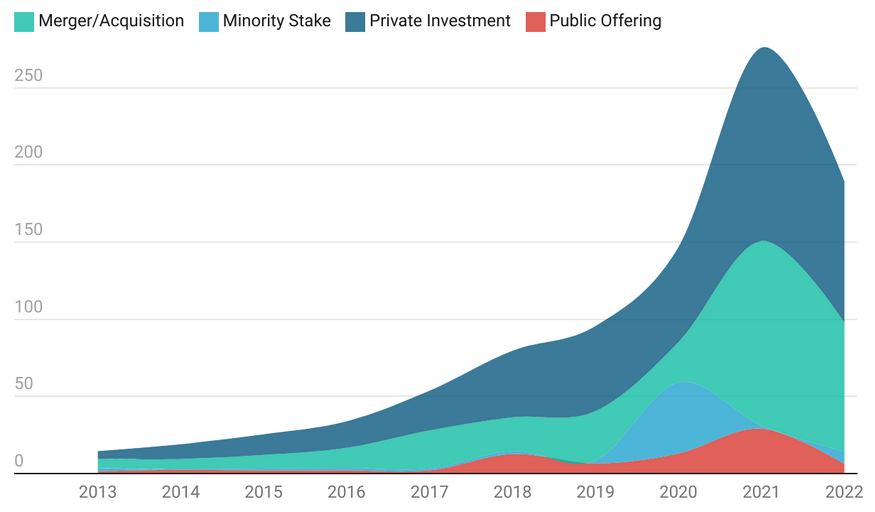
\includegraphics[width=\textwidth]{ai-investement.png}
    \caption{Inversión global en IA en miles de millones \cite{Letzing2024-nn}.}
    \label{fig:ai-investement}
\end{figure}

Nos encontramos en un momento en el que la demanda de equipos cualificados 
que puedan hacer frente a los nuevos desafíos es mayor que nunca. La complejidad
de los proyectos de IA también está en aumento, ya que las aplicaciones de IA
se vuelven más sofisticadas, abarcan una gama más amplia de funciones, requieren
un mayor número de datos y los modelos se vuelven cada vez más complejos. Esta
situación a forzado a las empresas a buscar nuevas formas de gestionar sus proyectos
que han llevado a la creación de nuevas metodologías, adaptadas a las necesidades
a los nuevos retos que se presentan. Si bien es cierto que mucha información es
compartida con la comunidad, existe un gran secretismo en torno a la forma de operar
de las empresas más grandes, lo que dificulta la adopción de estas metodologías.
Podemos resaltar positivamente el caso de Meta \cite{metaia}, que es el mayor 
referente en cuanto contribución y apertura de sus desarrollos en IA.\medskip

Por todo ello, es necesario realizar contribuciones que se centren en el como 
se debería operar dentro de un equipo. Se requiere de una referencia clara sobre las 
directrices que se deben aplicar para poder implementar un estándar tecnológico y
operacional dentro de un grupo de trabajo, así como las herramientas, metodologías y buenas prácticas
a seguir para hacer un uso eficiente de los recursos y obtener resultados de calidad.
Este documento representa un estándar que se ha aplicado en base a unas necesidades
concretas y, aunque no está pensado para poder ser adoptado de forma literal por otros equipos,
se muestra el camino que se ha seguido desde la adopción de plataformas MLOps hasta la creación
de un sistema de conocimiento para la reutilización de trabajo. La justificación de este
documento es exponer el trabajo realizado y servir como referencia equipos que quieran implementar
un estándar similar o busquen inspiración para crear el suyo propio.
 
%% Antecedentes -> Contenido general
%% Estado del arte -> Contribuciones de otros equipos
%% Referencias sobre replicabilidad 

\subsection{Antecedentes}
En la sección de antecedentes, se profundiza en aquellos conceptos esenciales que son 
indispensables para entender el alcance y las contribuciones de este trabajo, así como 
para situarlo dentro de un marco conceptual adecuado. Se abordan aspectos fundamentales 
que no solo proporcionan contexto, sino que también establecen las bases teóricas y 
metodológicas sobre las cuales se construye la investigación.

\subsubsection{Diseño Atómico}
El diseño atómico es una metodología de diseño que se centra en la creación
de sistemas modulares y reutilizables. La idea principal es dividir
las diferentes funcionalidades de un sistemas en sus partes más fundamentales,
de manera que cada una de estas partes pueda ser reutilizada en diferentes
contextos. Este enfoque permite tener un mayor control sobre cada una de las
partes del sistema, facilitando su mantenimiento, documentación y reutilización.
Originalmente, el diseño atómico ha sido aplicado en el diseño de interfaces
de usuario, pero su filosofía puede ser aplicada a cualquier sistema de diseño
modular. En el contexto de este proyecto, el diseño atómico se aplicará al
diseño de un sistema de componentes para el desarrollo de modelos de aprendizaje
automático.\medskip

Dentro del diseño atómico, los componentes se dividen en cinco categorías
principales, que representan diferentes niveles de abstracción. Estas categorías
son: átomos, moléculas, organismos, plantillas y páginas. Cada una de estas
categorías representa un nivel de abstracción diferente, y se relaciona con
las demás categorías de manera jerárquica. La figura \ref{fig:atomic-design}
muestra la estructura conceptual del diseño atómico. 

\begin{figure}[ht]
    \centering
    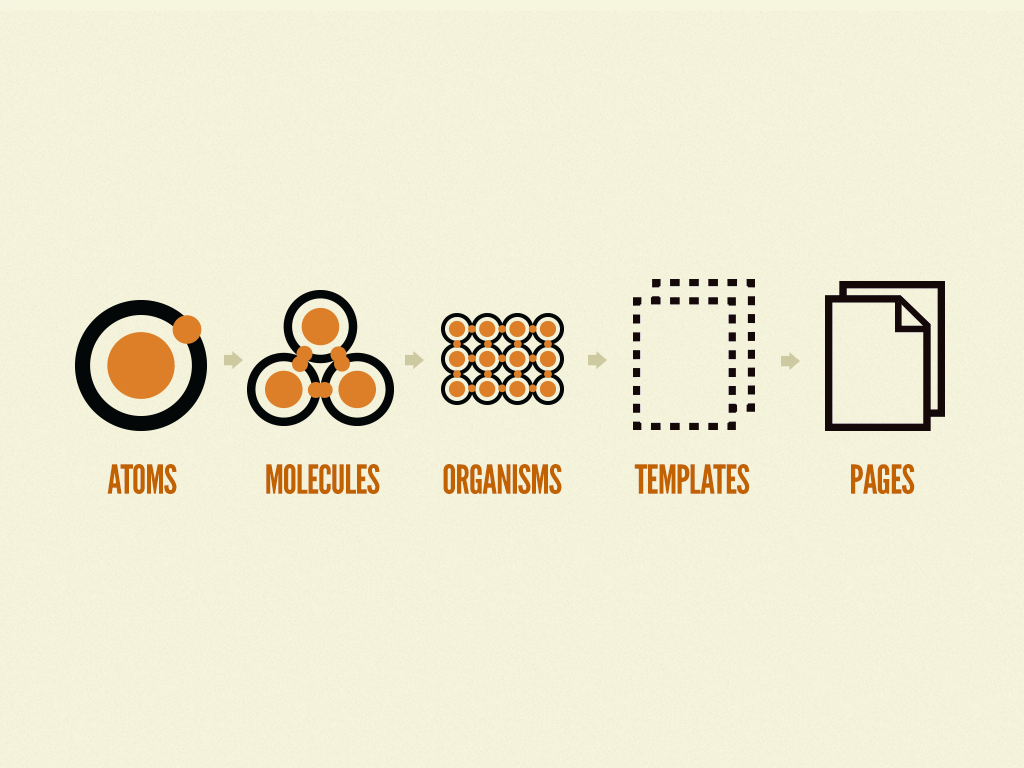
\includegraphics[width=0.7\textwidth]{atomic-design-process.png}
    \caption{Estructura conceptual diseño atómico \cite{frost2016atomic}.}\label{fig:atomic-design}
\end{figure}

A continuación, se describen brevemente cada una de las categorías:
\begin{itemize}
    \item \textbf{Átomos:} Los átomos son los componentes más básicos de un sistema
    de diseño. Representan las funcionalidades más fundamentales, solo tienen
    una responsabilidad y no dependen de otros componentes.
    \item \textbf{Moléculas:} Las moléculas son la combinación de varios átomos
    para formar una funcionalidad más compleja. Representan la combinación de
    diferentes funcionalidades básicas para formar una funcionalidad más compleja.
    \item \textbf{Organismos:} Los organismos son la combinación de varias moléculas
    y átomos para formar una funcionalidad completa.
    \item \textbf{Plantillas:} Las plantillas son la combinación de varios Organismos
    para dar forma a un contenido.
    \item \textbf{Páginas:} Las páginas son la combinación de varias plantillas.
\end{itemize}

Esta estructura jerárquica permite que los componentes sean reutilizados en
diferentes contextos, y que cada uno de ellos pueda ser modificado de manera
independiente. Además, se facilita la documentación y el mantenimiento de los
componentes, ya que cada uno de ellos es independiente de los demás. Podemos
ver multitud de ejemplos de diseño atómico en grandes empresas y que nosotros utilizamos
a diario, como por ejemplo en la creación de sistemas de diseño Microsoft Fluent
Design o Google Material Design entre otros.\medskip

Aunque el diseño atómico se ha aplicado tradicionalmente a la creación de interfaces
de usuario, su filosofía puede ser aplicada a cualquier sistema de diseño modular.
En el contexto de este proyecto, el diseño atómico se aplicará para la creación de un
sistema de componentes en el desarrollo de modelos de aprendizaje automático.
Traeremos la filosofía del diseño atómico y la adaptaremos a nuestro contexto,
con las particularidades y necesidades que requiere el desarrollo de modelos de
aprendizaje automático. 

\subsubsection{Machine Learning Operations (MLOps)}
El desarrollo de modelos de aprendizaje automático es un proceso complejo que implica
la recopilación de datos, la creación de modelos, la evaluación de los modelos y su
puesta en producción. Cada una de estas etapas requiere de diferentes herramientas y
prácticas, y es importante que estas herramientas y prácticas estén integradas de manera
coherente para garantizar la eficacia del proceso. Los principios de MLOPs son una serie de prácticas y herramientas que se utilizan
para gestionar el ciclo de vida de los modelos de aprendizaje automático. Como se muestra en la
figura \ref{fig:mlops-workflow}, este enfoque busca aplicar las mejores tendencias dentro de la 
ingeniería de software al desarrollo de modelos, con el objetivo de mejorar la eficiencia, la 
calidad y la escalabilidad.\medskip

\begin{figure}[ht]
    \centering
    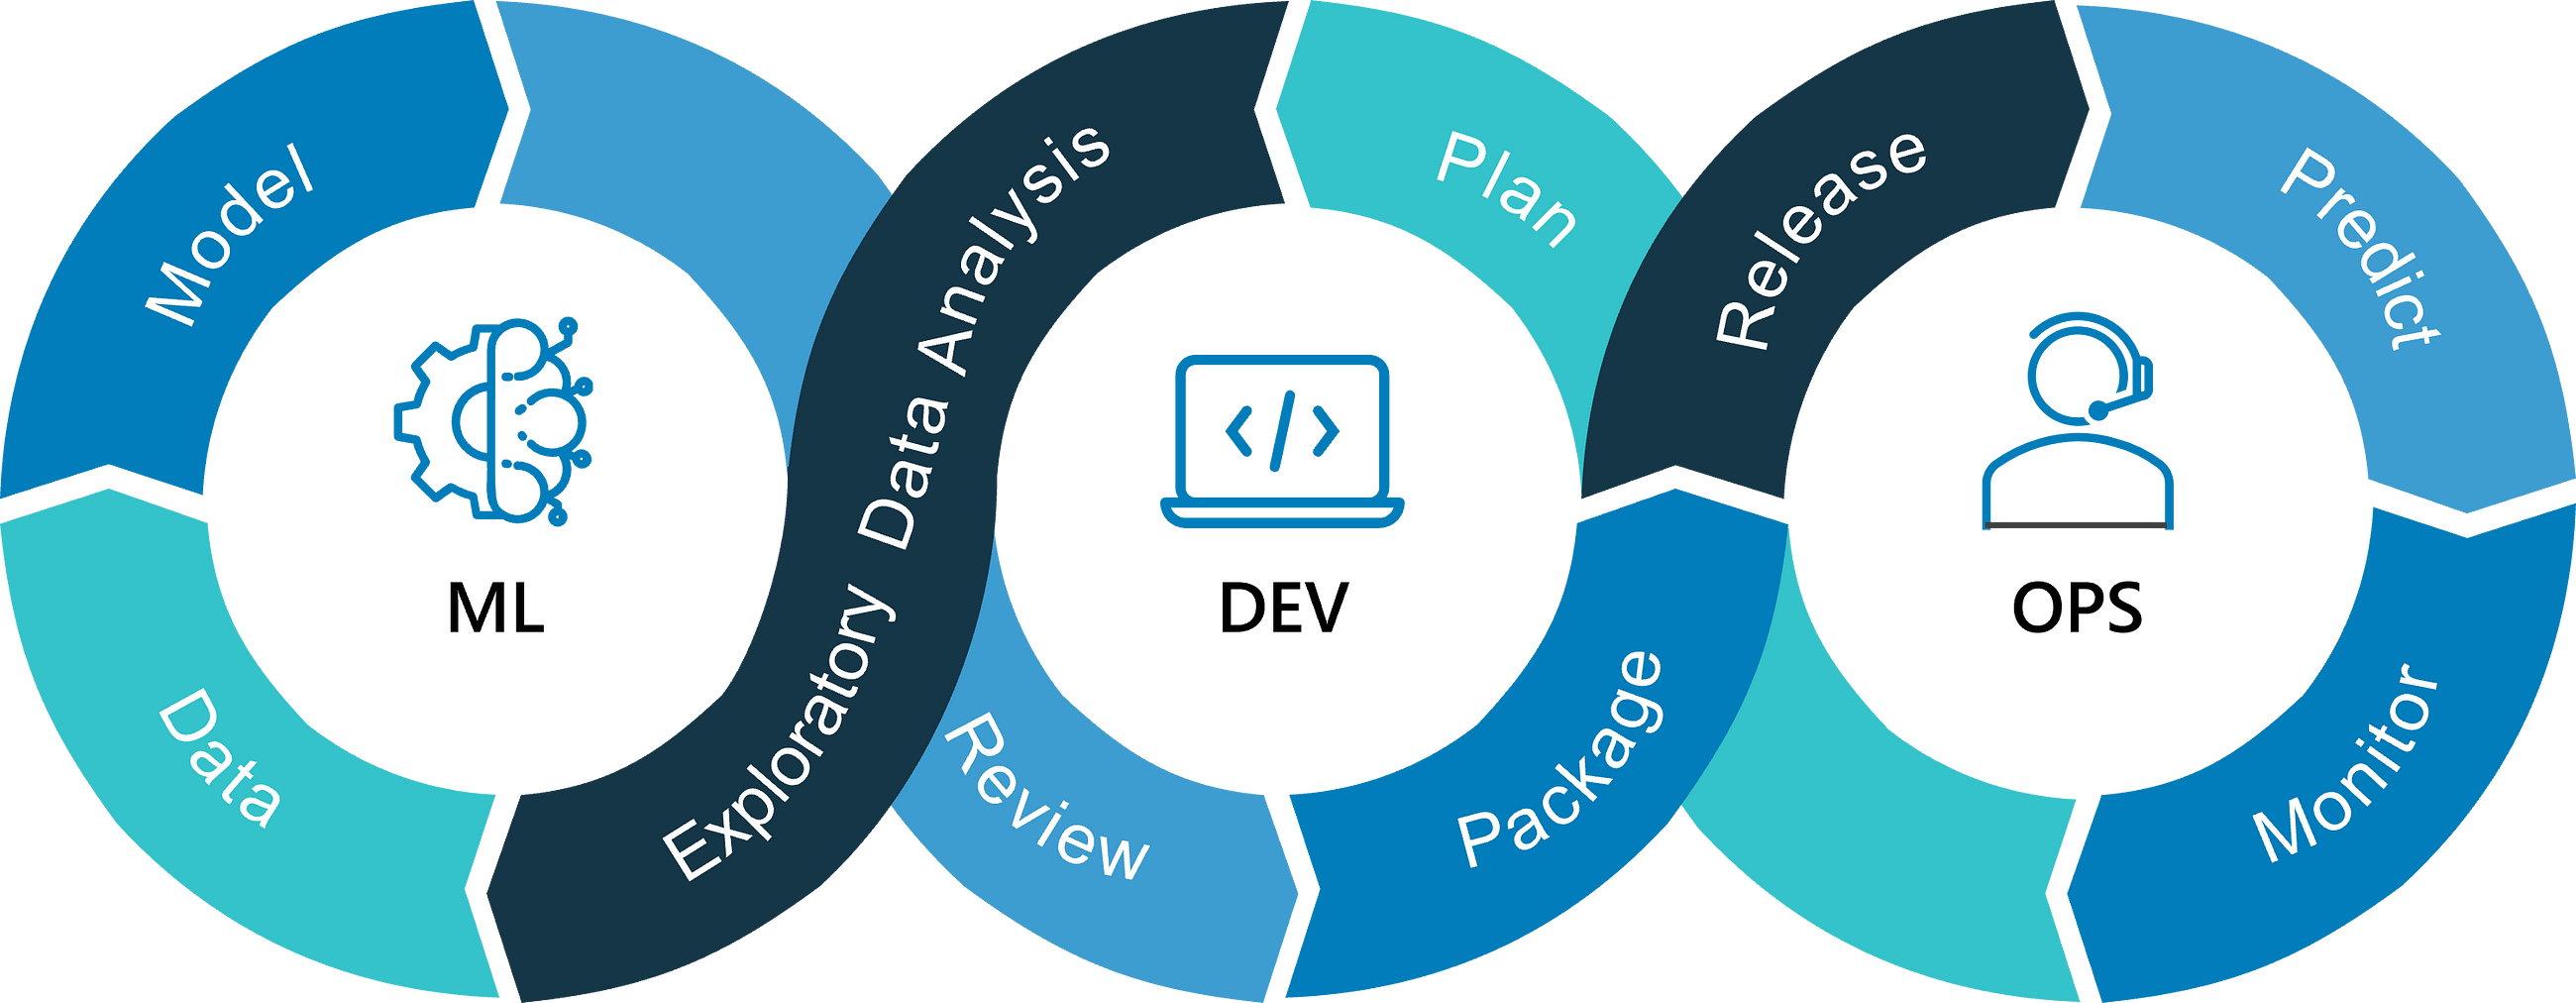
\includegraphics[width=\textwidth]{mlops-workflow.png}
    \caption{Ciclo de vida MLOps}\label{fig:mlops-workflow}
\end{figure}


Algunos de los principios clave de MLOps son:

\begin{itemize}
    \item \textbf{Automatización:} la automatización es esencial para mejorar la eficiencia del
    desarrollo de modelos y prevenir errores. Esto implica automatizar tareas como la 
    generación de datos, el despliegue de modelos, evaluación y su puesta en producción.
    \item \textbf{Colaboración y reproducibilidad:} uno de los desafíos en el Aprendizaje Automático es lograr 
    reproducir resultados de manera consistente, dada la naturaleza aleatoria de los algoritmos.
    MLOps busca, en la medida de lo posible, garantizar cierta consistencia entre los resultados
    obtenidos durante diferentes ejecuciones de un modelo para facilitar la colaboración entre
    los miembros del equipo.
    \item \textbf{Monitorización:} una vez que un modelo está en producción, es importante monitorizar
    su rendimiento para garantizar su eficacia y detectar posibles problemas. La monitorización
    permite crear alertas en caso de que el modelo no funcione correctamente y tomar medidas
    para corregirlo como por ejemplo, actualizar el modelo con nuevos datos.
    \item \textbf{Gestión de versiones:} controlar las versiones de los modelos y los datos es esencial
    para garantizar la reproducibilidad y la trazabilidad de los modelos. La gestión de versiones
    permite a los equipos comprender cómo ha evolucionado un modelo a lo largo del tiempo e incluso
    retroceder a versiones anteriores fuera necesario.
\end{itemize}

\subsection{Estado del arte}
La sección de estado del arte se centra en recopilar información sobre las tendencias
actuales dentro del ámbito del aprendizaje automático y la inteligencia artificial.
Debido a la diversidad de ramas que abarca la creación de un estándar tecnológico y
operacional, se han seleccionado aquellas que se consideran más relevantes o presentan
un mayor peso en cuanto a la toma de decisiones.

\subsubsection{Irrupción de las metodologías ágiles}
La aparición de metodologías ágiles en el desarrollo de software, con sus numerosas ventajas, 
ha dejado en desuso muchas metodologías clásicas. Las metodologías ágiles introdujeron el 
concepto de DevOps como un cambio de mentalidad \cite{salvucci2021mlops} 
en la que los diferentes equipos colaboran para implementar procesos más rápidos y 
entregar nuevas funcionalidades al cliente de manera más ágil. MLOps es una extensión de 
DevOps que ha surgido muy recientemente y, por lo tanto, existen pocos estudios que 
aborden el tema \cite{kreuzberger2022mlops}\cite{recupito2022multivocal}.\medskip

Principalmente existen dos formas para implementar MLOps en una organización, uno es
a través de los sistemas cloud que ofrecen servicios MLOps como Azure ML \cite{microsoft2023azureml}, 
AWS Sagemaker \cite{aws_sagemaker} o Google Cloud Vertex AI \cite{google2023vertexai}. El otro es a través del despliegue de una plataforma open source
como MLFlow dentro de la infraestructura propia. Las principales diferencias entre ambas
opciones son el coste y la flexibilidad, ya que los servicios cloud ofrecen una mayor
facilidad de uso y mejor experiencia de desarrollo, pero a un coste mayor. Por otro lado,
la implementación de una plataforma open source requiere de un mayor esfuerzo pero ofrece
se recompensa con una mayor flexibilidad y control sobre la infraestructura.

\subsubsection{Problemas de replicabilidad}
La crisis de replicabilidad es un fenómeno crítico en la comunidad científica,  
donde los resultados de los estudios a menudo no pueden replicarse con nuevos datos \cite{puetz2024replication}.
Este problema es muy destacado en numerosos campos científicos, que se han enfatizado particularmente 
en disciplinas como la psicología, la salud y la medicina \cite{puetz2024replication}\cite{Baker_2016}, donde hallazgos incorrectos 
podrían tener consecuencias graves. Durante los últimos años, la crisis de replicabilidad ha
sido objeto de debate dentro de la rama de la inteligencia artificial, donde la falta de
transparencia, la complejidad de los modelos y la imposibilidad de replicar los resultados
han sido identificados como problemas clave.

\begin{figure}[ht]
    \centering
    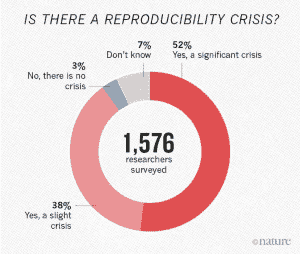
\includegraphics[width=0.75\textwidth]{crisis-survey.png}
    \caption{Encuesta a 1500 investigador sobre la reproducibilidad en la ciencia \cite{Baker_2016}}\label{fig:crisis-survey}
\end{figure}

La confusión se ve incrementada por el uso variado de términos clave como reproducibilidad, 
replicabilidad y repetibilidad, \cite{readytensor} dificultando los esfuerzos para abordar estos problemas de 
manera efectiva. Se definen los diferentes términos de la siguiente manera:
\begin{itemize}
    \item \textbf{Repetibilidad:} se centra en la consistencia de los resultados de la investigación cuando el equipo 
    original re-ejecuta su experimento bajo condiciones inalteradas. 
    \item \textbf {Reproducibilidad:} se logra cuando investigadores independientes validan los hallazgos del 
    experimento original empleando el documentado original. Esta validación puede ser directa, utilizando 
    los datos y el código originales, o independiente, a través de la reimplementación del experimento, 
    probando así la fiabilidad de los resultados en diferentes equipos.
\end{itemize}

Una serie de estudios y encuestas subrayan la gravedad de la situación \cite{Baker_2016}.
Como se muestra en la figura \ref{fig:crisis-survey}, una encuesta realizada a 1500 investigadores
encontró que el 50\% de ellos afirman que que hay una crisis significativa y un 40\% que hay
una crisis moderada, dejando solo un 10\% que no ve una crisis en la replicabilidad de los estudios.
Existen multitud de casos donde los intentos de volver a ejecutar experimentos dan como resultado 
a una amplia desviación, incluso bajo condiciones idénticas\ref{fig:crisis-survey}.
Los propios investigadores tienen dificultades para reproducir sus propios experimentos.
La figura \ref{fig:self-reproduce} nos da una idea de lo frecuente que es este problema,
donde en el caso de la física e ingeniería, el 50\% de los encuestados han tenido problemas
reproduciendo sus experimentos, lo que se ve reflejado en que el 70\% de ellos haya tenido
problemas al intentar reproducir los experimentos de otros investigadores.

\begin{figure}[ht]
    \centering
    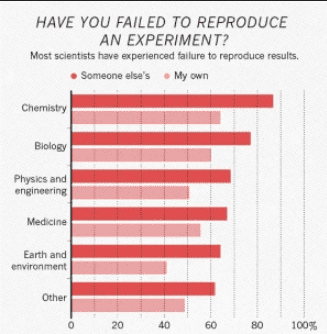
\includegraphics[width=\textwidth]{self-reproduce.png}
    \caption{Problemas con la reproducibilidad por disciplina \cite{Baker_2016}}\label{fig:self-reproduce}
\end{figure}

Estos problemas se consideran como los principales causantes como se puede ver en la figura \ref{fig:repro-factor}.
Factores como la falta de información sobre detalles experimentales y los tiempos de publicación, enfatizando 
la necesidad urgente de un enfoque más sistemático y transparente. Sin contar los problemas
directamente relacionados con el desarrollo, como son la procedencia y calidad de los datos, la 
elección del algoritmo, el hardware utilizado para su entrenamiento, el preprocesamiento de 
los datos, entre otros.

\begin{figure}[ht]
    \centering
    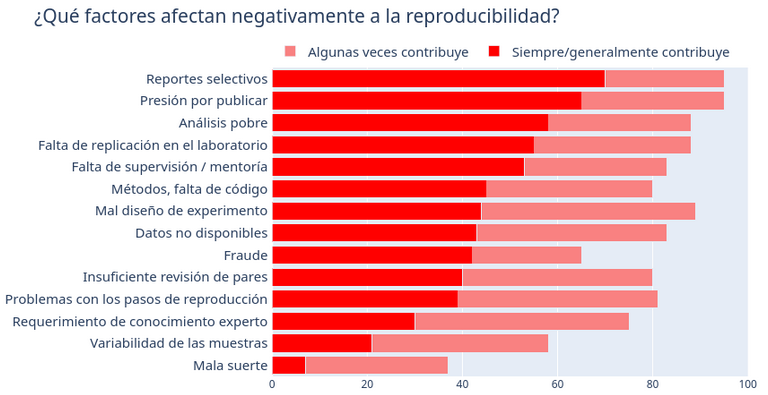
\includegraphics[width=0.5\textwidth]{repro-factor.png}
    \caption{Factores que contribuyen a la irrepoducibilidad \cite{Baker_2016}}\label{fig:repro-factor}
\end{figure}

Aunque la crisis de un problema complejo y multifacético, existen
algunas medidas que pueden tomarse para abordarlo. Algunas de estas medidas que encontramos
en al literatura son un mejor supervisión, mejora del proceso de validación, incentivar
buenas practicas de desarrollo, entre otras

\subsubsection{Calidad del software y buenas prácticas}


\pagebreak
    \section{Objetivos y alcance}
En esta sección se introducen los objetivos del 
proyecto, habiéndose realizado una division entre el principal y los
secundarios. Ademas de ello, se presentan los elementos que forman el alcance,
asi como se comentan otros que no.

\subsection{Objetivos generales}
El objetivo principal del proyecto es diseñar e implementar un estándar tecnológico y 
operacional que cubra las necesidades más comunes dentro de un equipo de \textit{data science}. Se 
busca agilizar los tiempos de desarrollo y estandarizar los procesos, con el fin de
facilitar la colaboración entre investigadores y la reutilización del conocimiento. A
continuación, se detallan los objetivos específicos que guiarán el desarrollo:

\begin{itemize}
    \item \textbf{Agilizar el proceso inicial de proyectos:} Optimizar las primeras etapas 
    de los proyectos, identificando y eliminando aquellos procesos repetitivos que no aportan
    valor y que puedan retrasar su puesta en marcha. 
    \item \textbf{Facilitar la colaboración entre investigadores:} Implementar herramientas y 
    métodos que fomenten una cooperación fluida y efectiva entre los miembros del equipo de 
    investigación, con el fin de potenciar la sinergia y aprovechar al máximo el conocimiento 
    colectivo.
    \item \textbf{Definir procesos mediante buenas prácticas:} Establecer un marco de trabajo 
    basado en buenas prácticas de gestión de proyectos, con el objetivo de estandarizar los 
    procesos y garantizar su eficiencia y calidad.
    \item \textbf{Automatizar el desarrollo de modelos robustos:} Investigar y aplicar 
    técnicas que contribuyan al desarrollo automático de modelos de aprendizaje automático,
    con el fin de reducir el tiempo y el esfuerzo necesarios para obtener resultados de calidad.
    \item \textbf{Promover la reutilización del conocimiento:} Desarrollar mecanismos y herramientas 
    que faciliten la captura, organización y difusión del conocimiento generado durante el desarrollo 
    de los proyectos, con el propósito de fomentar su reutilización en futuras investigaciones y 
    actividades relacionadas.
\end{itemize}

El cumplimiento de estos objetivos se espera que no solo mejore la eficiencia y la calidad de los 
proyectos, sino que también contribuya a la creación de un entorno de trabajo más colaborativo y
enriquecedor para los miembros del equipo de investigación.

\subsection{Alcance}
En esta sección se definen los límites del proyecto, estableciendo lo que está
incluido y excluido dentro mismo. Se describirá de manera detallada las
actividades que forman parte del desarrollo final, así como aquellos elementos
que no están incluidos en el alcance del proyecto. Aunque el enfoque de este 
proyecto podría aplicarse a una amplia variedad de problemas en el ámbito del 
aprendizaje automático, en el contexto de este TFM nos centraremos en tres de 
los casos más comunes dentro del marco de las series temporales: Forecasting, 
Clasificación y Detección de Anomalías. A continuación, se detallan las 
actividades que forman parte del alcance del proyecto.

\subsubsection{Dentro del alcance}
\begin{itemize}
    \item \textbf{Integración de sistemas externos:} Se incluirá la configuración de sistemas 
    externos, como plataformas MLOPs o herramientas de visualización, con las plantillas 
    de proyectos base. Esto permitirá una integración más fluida y rápida de estos sistemas con 
    los proyectos, facilitando el flujo de datos y la visualización de resultados.
    \item \textbf{Plantillas de proyectos base:} Desarrollar plantillas para 
    los tres problemas de series temporales comentados anteriormente. Estas plantillas 
    servirán como punto de partida para proyectos específicos dentro de cada uno de estos dominios
    y definirán desde el principio una estructura y un conjunto de herramientas comunes. Además,
    se incluirán ejemplos de código y documentación que faciliten su uso y comprensión.
    \item \textbf{Componentes esenciales:} Identificar y almacenar los componentes 
    esenciales de cada proyecto, incluyendo modelos, algoritmos, métricas de evaluación y
    preprocesamiento de datos. Estos componentes se almacenarán y documentarán de forma
    que puedan ser reutilizados en futuros proyectos, facilitando la transferencia de conocimiento.
    \item \textbf{Proceso de AutoML:} Diseñará y ejecutar procesos de AutoML 
    (Machine Learning Automatizado) que demostrará cómo se pueden combinar los conocimientos 
    adquiridos de todos los proyectos para desarrollar un sistema de aprendizaje automático 
    automatizado. Este proceso utilizará las plantillas y componentes esenciales almacenados 
    para generar modelos de forma automática.
\end{itemize}

\subsubsection{Fuera del alcance}
\begin{itemize}
    \item \textbf{Desarrollo de modelos específicos:} Aunque se incluirán ejemplos de
    modelos y algoritmos, el desarrollo de modelos específicos para problemas concretos
    no forma parte del alcance de este proyecto. Se espera que los modelos desarrollados
    sean generales y puedan ser adaptados a problemas específicos por los usuarios.
    \item \textbf{Despliegue de modelos:} El despliegue de modelos en producción no forma
    parte del alcance de este proyecto. Se espera que los modelos desarrollados puedan ser
    desplegados en sistemas de producción, pero no se incluirá en este proyecto. El enfoque
    se centrará exclusivamente en el desarrollo de los mismos.
\end{itemize}

\pagebreak
    \section{Metodología del Proyecto}
En esta sección, se describirá la metodología para abordar tanto el
desarrollo del software como la propia metodología de investigación. La metodología
de desarrollo de software se basa en el uso de metodologías ágiles \cite{Agile_Microsoft}, concretamente
en la metodología Scrum \cite{Atlassian_Scrum}. Por otro lado, la metodología de investigación es una
metodología propia diseñada para abordar problemas dentro del marco de trabajo de
los problemas combinatorios NP-Hard diseñada por el autor de este trabajo. Esta
metodología se basa en el uso de técnicas de IL.

\pagebreak 
    \section{Conclusiones y trabajo a futuro}
En esta sección se presentan las conclusiones obtenidas tras la finalización 
del proyecto, así como las lecciones aprendidas y los conocimientos adquiridos. 
Además, se presentan ideas o propuestas que podrían ser utilizadas o implementadas 
en el futuro para mejorar o ampliar el alcance del proyecto.

\subsection{Conclusiones}
Una vez finalizado el proyecto, se presentan las siguientes conclusiones en 
base a los resultados obtenidos y analizados durante el desarrollo del mismo.
Estas representan los cuatro aspectos clave del proyecto: reducción del tiempo de desarrollo, 
mejora de la productividad, reutilización del conocimiento y colaboración. Estas conclusiones 
reflejan los beneficios tangibles que el marco tecnológico propuesto aporta a los 
equipos y sus proyectos.\medskip

La implementación ha demostrado ser eficaz en la reducción significativa del tiempo 
de de\-sarro\-llo. Al automatizar tareas repetitivas y procesos manuales, se liberan 
recursos y se acelera el progreso de los proyectos. La adopción de metodologías 
ágiles y MLOps permite responder rápidamente a los cambios del entorno empresarial, 
proporcionando una ventaja competitiva crucial en cuanto a tiempo se refiere. La 
integración de plataformas como ClearML y Rath facilita la gestión y 
monitorización de experimentos, lo que reduce el tiempo dedicado a la configuración 
y gestión manual de estos procesos.\medskip

La mejora de la productividad es uno de los beneficios más destacados de la 
implementación del marco tecnológico. La automatización de tareas y la 
estandarización de procesos permiten a los equipos centrarse en actividades 
de mayor valor añadido. Además, el uso de herramientas de colaboración y la 
integración de sistemas de gestión del conocimiento aseguran que la información 
se comparta y reutilice de manera efectiva. Esto no solo incrementa la eficiencia 
operativa, sino que también mejora la calidad del trabajo, ya que los investigadores 
pueden dedicar más tiempo a la innovación y menos a tareas repetitivas.\medskip

El diseño de un sistema de componentes reutilizables y plantillas base para 
proyectos específicos facilita la reutilización del conocimiento adquirido. 
La creación de un catálogo de componentes esenciales y la documentación exhaustiva 
del proyecto aseguran que las mejores prácticas y soluciones previas se 
puedan aplicar en futuros proyectos. Este enfoque modular y estandarizado no 
solo ahorra tiempo, sino que también mejora la coherencia y calidad de los 
desarrollos, permitiendo a los equipos construir sobre trabajos anteriores 
de manera más eficiente.\medskip

La adopción de un marco común y la integración de herramientas colaborativas 
son fundamentales para mejorar la cooperación entre los miembros del equipo. 
La estandarización de procesos y la implementación de sistemas de autenticación 
y seguridad, como Keycloak, garantizan un entorno seguro y accesible para todos 
los miembros del equipo. Además, la encuesta de satisfacción realizada a los
miembros del equipo ha sido acogida de manera positiva, lo que sugiere que
existe un interés y una aceptación generalizada del nuevo marco tecnológico.\medskip

En conclusion, en base a los resultados obtenidos y analizados durante el desarrollo
del proyecto, se puede afirmar que la implementación del marco tecnológico propuesto
ha sido exitosa. Los beneficios tangibles obtenidos son muy positivos y sugieren que
el uso de este marco tecnológico puede mejorar significativamente la eficiencia y
productividad de los equipos.

\subsection{Trabajo a futuro}
A continuación, se presentan las siguientes propuestas de mejora y ampliación
del proyecto que podrían ser implementadas en futuras iteraciones:

\begin{itemize}
    \item \textbf{Adaptación del sistema a visión por computador:} Actualmente, la infraestructura 
    está enfocada en problemas basados en series temporales, pero se podría ampliar
    su alcance para incluir problemas de visión por computador. Se podría implementar
    no solo funcionalidades de preprocesamiento de imágenes, sino también incluir
    plataformas de etiquetado de imágenes populares como Cvat \cite{CVAT} o incluso conectar el
    sistema de versionado de datasets con herramientas como FiftyOne \cite{FiftyOne}.
    \item \textbf{Integración de ClearML con las tarjetas gráficas de la empresa:} Para 
    optimizar el uso de recursos de cómputo, se propone conectar ClearML con las 
    gráficas (GPUs) de la empresa. Esta integración permitirá gestionar y monitorear las 
    tareas de procesamiento de manera eficiente, asegurando una distribución adecuada de las 
    cargas de trabajo. ClearML facilitará la asignación dinámica de recursos, mejorando 
    la eficiencia del procesamiento y reduciendo tiempos de espera. Se podría implementar un 
    sistema de colas que divida las tareas según su prioridad y requerimientos de recursos. 
    Esto incluiría la creación de diferentes colas para tareas de alta prioridad, 
    tareas de procesamiento intensivo y tareas de mantenimiento. ClearML gestionaría estas colas, 
    asignando las tareas a las GPUs disponibles y asegurando un uso equilibrado y eficiente de los recursos.
    \item \textbf{Monitorización y análisis de rendimiento:} Implementar herramientas de monitorización 
    que proporcionen métricas detalladas sobre el uso de los recursos, el rendimiento de las 
    tareas y la eficiencia del sistema en general. Estas herramientas permitirían identificar 
    cuellos de botella, optimizar la asignación de recursos y planificar mejoras futuras 
    basadas en datos concretos. Además, se podría implementar un sistema de alertas que
    notifique sobre posibles problemas o anomalías en el rendimiento del sistema, permitiendo
    una respuesta rápida y eficaz ante situaciones críticas.
\end{itemize} 
    \pagebreak 
    \printbibliography[title=Bibliografía]
    \pagebreak
\end{document}